% Created 2017-05-20 lör 10:58
% Intended LaTeX compiler: pdflatex
\documentclass[11pt]{article}
\usepackage[utf8]{inputenc}
\usepackage[T1]{fontenc}
\usepackage{graphicx}
\usepackage{grffile}
\usepackage{longtable}
\usepackage{wrapfig}
\usepackage{rotating}
\usepackage[normalem]{ulem}
\usepackage{amsmath}
\usepackage{textcomp}
\usepackage{amssymb}
\usepackage{capt-of}
\usepackage{hyperref}
\addtolength{\textwidth}{5cm}
\addtolength{\textheight}{4cm}
\addtolength{\hoffset}{-2.5cm}
\addtolength{\voffset}{-2.5cm}
\author{Sebastian Heimlén}
\date{\today}
\title{Displaimer Projektdefinition}
\hypersetup{
 pdfauthor={Sebastian Heimlén},
 pdftitle={Displaimer Projektdefinition},
 pdfkeywords={},
 pdfsubject={},
 pdfcreator={Emacs 25.1.1 (Org mode 9.0.5)}, 
 pdflang={Swedish}}
\begin{document}

\maketitle
\begin{abstract}
Detta dokument är en projektdefinition (Eklund, 2010) för studentprojekt eller examensarbete vid KTH ICT.

En projektdefinition är inte en projektplan utan föregår ofta en sådan. Projektdefinitionen kan
vid behov utvecklas till en projektplan. För examensarbetet är det lämpligt att projektdefinitionen
fungera som ”överenskommelse” mellan projektets huvudintressenter vilka oftast är ett företag, studenten
som gör arbetet och akademin varifrån studenten kommer. Förändras projektet i något viktigt avseende
så uppdateras och förankras projektdefinitionen.
\end{abstract}


\section*{Dokumentversion}
\label{sec:orgc9297a6}
\begin{center}
\begin{tabular}{rlll}
\textbf{Datum} & \textbf{Version} & \textbf{Författare} & \textbf{Beskrivning}\\
\hline
2017-03-22 & Version 1.0 & Sebastian Heimlén & Första utkastet.\\
2017-04-06 & Version 1.1 & Sebastian Heimlén & Första revidering.\\
2017-05-08 & Version 1.2 & Sebastian Heimlén & Uppfräschning efter sprint \#3.\\
2017-05-13 & Version 1.3 & Teo Klestrup Röijezon & Diverse layoutändringar\\
2017-05-19 & Version 1.4 & Sebastian Heimlén & Uppdatering efter sprint \#4.\\
\end{tabular}
\end{center}


\pagebreak
\setcounter{tocdepth}{4}
\tableofcontents

\section{Introduktion}
\label{sec:org8fb627a}
\subsection{Dokumentets syfte}
\label{sec:org2176475}
Denna projektdefinition skall ge en övergripande beskrivning av varför,
hur och när detta projekt ska genomföras, samt även innehålla mer
specifik information gällande arbetsplan, riskanalys, förändringsplan,
kostnadsplan etc.

\subsection{Dokumentets omfattning}
\label{sec:orga004008}
Detta dokument behandlar följande:

\begin{itemize}
\item Hur projektet planeras att genomföras

\item Varför projektet planeras att genomföras

\item Vilka mål som slutligen ska uppnås med projektet, och varför dessa
mål är viktiga och/eller intressanta.
\end{itemize}

Detta dokument behandlar \emph{inte} följande:

\begin{itemize}
\item Specifika detaljer gällande det faktiska systemet som ska utvecklas,
så som systemets arkitektur.

\item Information om vilka programmeringsspråk eller/och ramverk som kommer
användas.

\item Tekniska detaljer om slutprodukten.
\end{itemize}

\subsection{Dokumentöversikt}
\label{sec:org7ca83ef}
Detta dokument innehåller följande delar:

\begin{itemize}
\item \textbf{Projekt- eller uppgiftsbeskrivning} -- detta görs översiktligt och
sammanfattande

\item \textbf{Organisation} -- hur arbetet och samarbete skall organiseras

\item \textbf{Projektmål} -- vilka är huvudintressenternas syfte/mål med
projektet? Varför är man med i detta projekt?

\item \textbf{Fas- och tidsplan} -- arbetsvolym, projektets varaktighet,
översiktlig fas och tidsindelning, flexibilitet i ”projekttriangeln”-
projektåtagande (resurser/kostnad-varaktighet(tid)-funktionalitet)

\item \textbf{Intressenter} -- vilka är projektets intressenter, deras
förväntningar och ambition att uppfylla dessa förväntningar och hur.

\item \textbf{Riskanalys} -- riskidentifiering och åtgärder. Hur hanteras
eventuell sekretess och konfidentialitet mm?

\item \textbf{Förändringsplan} -- hur hanteras och meddelas viktiga förändringar i
projektet?

\item \textbf{Kostnader} -- vilka kostnader finns i projektet? Vem betalar vad?
Licenser?

\item \textbf{Dokumentplan} -- vilka dokument skall användas, underhållas och
levereras?

\item \textbf{Utbildningsplan} -- behov av förstudie, inläsning, utbildning.

\item \textbf{Rapport- och granskningsplan} -- syfte och tider för rapportering
och granskning.

\item \textbf{Referenser} -- detaljerad referenslista enligt APA, Vancouver eller
annat (APA kan vara bra så länge man skriver för man ser författaren
och förstår då vilken källa det handlar om medans Vancouver ger ett
nummer som inte säger något)
\end{itemize}

\section{Projektöversikt -- bakgrund, syfte och mål}
\label{sec:org92adba0}
Detta kapitel ger en översikt av projektet.

\subsection{Bakgrund}
\label{sec:orgfd8ef3a}
Önskemålet som vår uppdragsgivare har är att denna vill ha en display på
sin kontorsdörr som denna person via en webbapplikation eller hemsida
ska kunna skriva in meddelanden på för att upplysa kollegor, kunder samt
besökare om denna persons nuvarande status, displayen skulle till
exempel kunna visa meddelandet ”sjuk, tillbaka på onsdag” eller ”möte
till 14:00”.

Vi som projektgrupp har även egna önskemål som ligger bakom detta
projekt, dels vill vi lära oss projektmetodik i allmänhet och
Scrum-metodiken i synnerhet, men detta projekt är även en stor del av en
kurs som vi läser på KTH som heter ”Projekt och Projektmetoder”. I denna
kurs skall vi genom litteraturstudie och praktiskt arbete undersöka
olika projektmetoder för att besvara frågeställningen ”Vad är en bra
projektmetod för små IT-projekt”. Denna frågeställning ska sedan
besvaras i en rapport som också är en del av examinationen i denna kurs.
Vi måste därför under projektets gång undersöka, diskutera samt dra
slutsatser kring vad vi tycker är bra projektmetoder i detta projekt,
som kan anses vara ett litet IT-projekt.

\subsection{Syfte}
\label{sec:orgf793aef}
Slutprodukten av projektet förväntas underlätta för både vår kund samt
dennes besökare, eftersom det kommer vara enkelt att skriva ut ett
beskrivande meddelande på skärmen som besökare och kollegor kan ta del
av, oavsett vart innehavaren av skylten befinner sig. Nuvarande lösning
är en whiteboard tavla, men detta kommer vara en stor förbättring då all
modifiering av skärmen sker digitalt, medan en whiteboard tavla kräver
att innehavaren faktiskt befinner sig i lokalen och fysiskt skriver in
meddelandet på skärmen.

Vårt syfte som projektgrupp är som tidigare nämnt att bli bättre på att
jobba i projekt, och lära oss diverse projektmetoder, detta är en
kunskap som vi kommer ha användning för i vårt följande yrkesliv, då en
väldigt stor del av IT-utveckling i dagens samhälle sker i projekt, och
just Scrum i synnerhet används i väldigt stor utsträckning.

Detta är också ett bra tillfälle att träna på att göra undersökningar
och sedan skriva en vetenskaplig text som förklarar och berättar om
dessa undersökningar, så som vi ska göra i kursrapporten som görs som en
direkt följd av detta projektarbete, eftersom vi senare kommer att göra
just detta när vi genomför examensarbetet i årskurs 3, så syftet med
detta projekt och tillhörande kursrapport är också delvis en
förberedelse för examensarbetet.

\subsection{Mål}
\label{sec:orgd9b463c}
\begin{itemize}
\item Skapa en webbapplikation som jobbar mot en databas.

\item Skapa nämnd databas

\item Köra denna webbapplikation på en Raspberry Pi

\item Koppla en elektronisk display mot ett kretskort som TIEDB studenterna
ritat.

\item Trådlöst koppla hallonpajen mot displayen, på så sätt att displayen
kan visa meddelanden som skrivs in i webbapplikationen.

\item Undersöka olika projektmetoder och bilda sig en uppfattning kring
dessa

\item Skriva ett antal formella dokument (olika dokument beroende på roll i
projekt)

\item Skriva en teknisk specifikation för en del i systemet som den
personen skapat (Varje medlem skriver en egen spec.)

\item Tillsammans skriva en rapport som besvarar frågeställningen ”Vad är
en bra projektmetod för små IT-projekt”, där vissa delar skrivs
enskilt baserat på roll i projektet.
\end{itemize}

\subsection{Funktionella krav - användningsfallsmodell}
\label{sec:org32f238d}
Detta diagram visar hur en användare går till väga när den vill nyttja
systemet.

\begin{center}
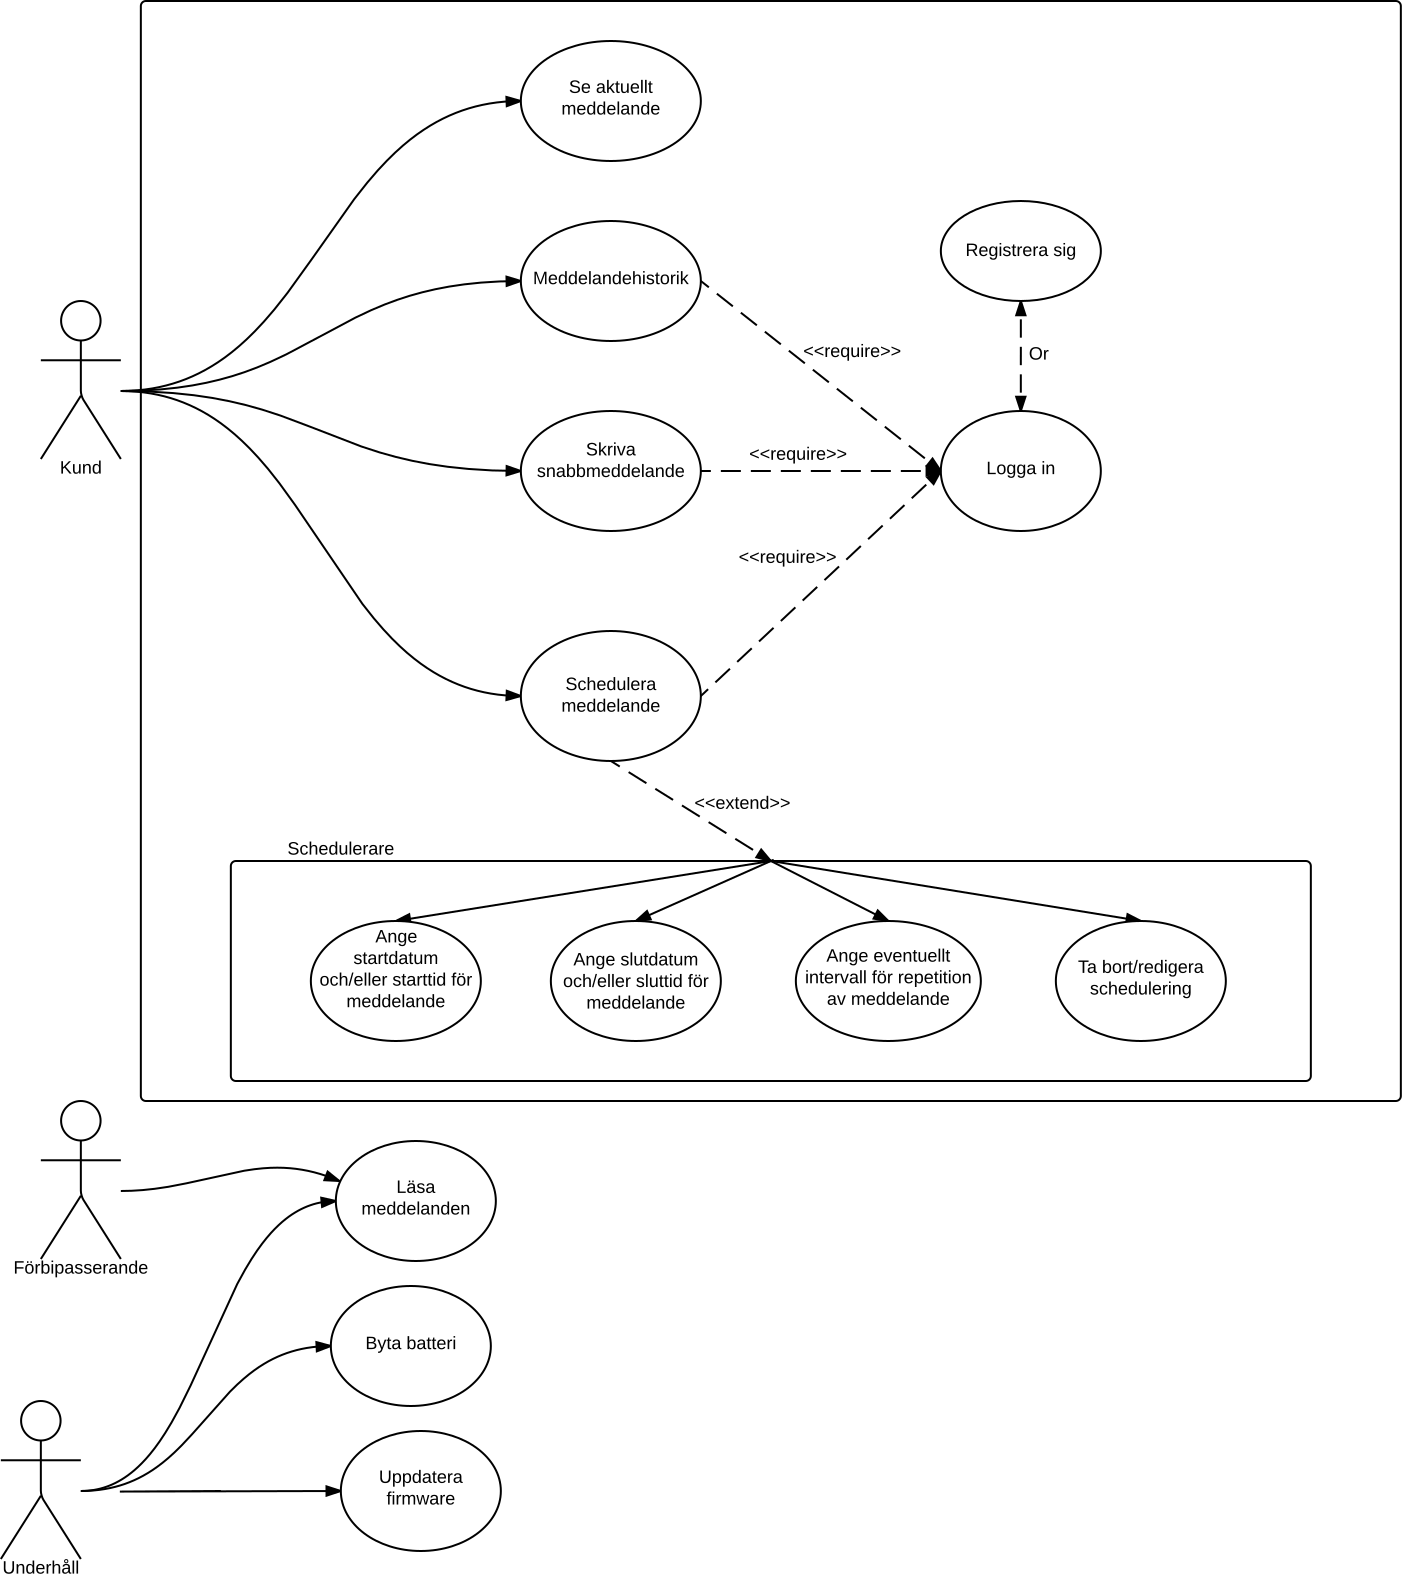
\includegraphics[width=.9\linewidth]{../Arkitektur/PrimarUC.png}
\end{center}

\section{Organisation}
\label{sec:org2a84e43}
\subsection{Personer i projektet}
\label{sec:org47e30ad}
\begin{center}
\begin{tabular}{ll}
\textbf{Namn} & \textbf{Kontaktuppgift och roll}\\
\hline
Teo Klestrup Röijezon & \href{mailto:teo@nullable.se}{\emph{teo@nullable.se}}, \href{mailto:roijezon@kth.se}{\emph{roijezon@kth.se}}\\
 & Arkitekt och Utvecklingsansvarig.\\
Yobart Amino & \href{mailto:yobart@kth.se}{\emph{yobart@kth.se}}\\
 & Testansvarig, arbetsmiljöansvarig\\
Henrik Björklund & \href{mailto:hebjo@kth.se}{\emph{hebjo@kth.se}}\\
 & Kund-/kravansvarig, shoppingansvarig\\
Sebastian Heimlén & \href{mailto:heimlen@kth.se}{\emph{heimlen@kth.se}}\\
 & Projektledare, etik och jämställdhetsansvarig\\
\end{tabular}
\end{center}

\subsection{Möten}
\label{sec:org8420447}
Ett antal möten i veckan kommer att hållas, samtliga dagar som har
schemalagda pass påbörjas med ett scrum möte, där gruppen går igenom vad
de enskilt har jobbat med den senaste dagen/dagarna och hur arbetet
skall fortskrida.

I början av varje sprint hålls ett sprintmöte. I detta möte kommer
kravansvarig att agera proxy för produktägaren. I sprintmötet bestäms
iterationsmålet för vidkommande sprint, utifrån detta iterationsmål
väljs use-case slices ut och tasks baseras på dessa slices, sedan
genomförs scrum-poker för att bestämma antal story-poäng vardera task
kommer att kosta, samt viktighetsgrad den innehar.

I slutet av varje sprint hålls ett retrospective-möte där projektgruppen
går igenom hur vi tycker att sprinten gått, vad som varit bra, vad som
varit mindre bra, vad som skall behållas till nästa sprint samt
eventuella saker som skall prövas i nästa sprint. Detta för att öka
kvalitén och förståelsen för projektet och arbetet, men också för att
alla i gruppen skall ha rum att yttra sina egna tankar och funderingar,
detta blir helt enkelt ett forum där samtliga medlemmar kan få saker
sagt och förändringar genomförda.

\subsection{Arbetsplats}
\label{sec:org5a41658}
Vi kommer de flesta dagar att sitta tillsammans i skolan, ofta på plan 3
då det har ställts ut många bord där 4 personer kan sitta och jobba
ihop. De dagar vi sitter och jobbar enskilt sitter vi hemma eller på
bibliotek eller liknande. Anledningen till att vi vill spendera så
mycket tid som möjligt i skolan tillsammans är för att det är enklare
att diskutera och komma fram till lösningar på problem om man
tillsammans i gruppen resonerar kring dessa, och detta görs enklast och
bäst i person och ej över internet.

\subsection{Arbetsutrustning}
\label{sec:orgb108a88}
Vi använder oss av ett tvåsidigt scrumboard, den ena sidan består av
Sprint backlogen där vi kan följa vårt arbete i sprinten, vilka stories
som är påbörjade, avslutade etc. På sprint backlogen finns också vår
burn down där vi kan följa vår progression. På den andra sidan återfinns
product backlogen, som kan ses som den publika sidan av scrumboarden,
det vill säga den sida som kunden och andra utomstående ur projektet kan
se vad projektgruppen åstadkommit hittills och hur arbetet fortlöper. Vi
använder oss också av Trello, som är en onlinetjänst som kan
konfigureras efter behov, vi har valt att konfigurera denna enligt
KanBan, det vill säga vi har ett fält ”checked out”, ett fält ”test”
samt ett fält ”done”. På Trello återfinns också samtliga use-case
slices, tasks samt test-cases, för samtliga sprints. På detta sätt
fungerar Trello både som en backup av tavlan, en historik över projektet
samt ett arbetsverktyg som kan användas vid aktuellt arbete.

\subsection{Meddelanden}
\label{sec:orgec838cb}
För att kommunicera med varandra och skicka meddelanden etc. när vi inte
träffas i skolan så använder vi gitter.im som är en
kommunikations-applikation som är kopplad till github, man loggar in med
sitt github konto och har sedan dels en chatt samt kan skapa olika
projekt och communities etc. Vi använder för nuvarande endast chatten
och resten av dokumenthanteringen överlåter vi till github.

\section{Projektets olika mål}
\label{sec:orgcc77bf6}
Vilka är de olika intressenternas mål med projektet?

Eklund (Eklund, 2010) anger tre olika typer av mål med ett projekt

\begin{itemize}
\item Effektmål

\item Resultatmål

\item Projektmål
\end{itemize}

Hur relaterar målen nedan till dessa? Vad är vad?

\subsection{Uppgiftsägaren}
\label{sec:orgd3f752b}
Vi planerar att använda oss av den agila projektmetodiken Scrum, en agil
metodik går ut på att man i slutet av varje sprint förväntas ha en
fungerande produkt, som sedan i vidkommande sprinter kan utvecklas, och
det är så vi planerar att jobba också, det vill säga att i slutet av
sprint \#2 hoppas vi att vi kan ha en, förvisso väldigt enkel, fungerande
produkt som vi i kommande sprinter kan vidareutveckla och addera mer
funktionalitet och komplexitet till.

Det konkreta projektmålet är att vi ska producera en webbapplikation som
är kopplad till en databas, på denna webbapplikation ska man kunna skapa
ett konto och logga in i applikationen, när man är inloggad i
applikationen ska man kunna skriva ett meddelande som sedan ska visas på
en elektronisk display. Denna display ska vara trådlöst ansluten till en
Raspberry pi där webbapplikationen körs. Detta resultatmål kommer leda
till att effektmålet, som är att vår kund på ett enkelt och portabelt
sätt ska kunna skriva ut information till kollegor och besökare, även om
vår kund inte själv är tillgänglig, kommer att uppfyllas.

\subsubsection{Effektmål}
\label{sec:org8a5fcc1}

Denna produkt kommer underlätta för vår uppdragsgivare samt för hans
kollegor och besökare, vår uppdragsgivare kommer nu ej behöva vara
närvarande på arbetsplatsen för att informera om varför/när han ej är
tillgänglig, detta kommer leda till mindre frustration hos kollegor samt
besökare, då de enklare kan planera sina besök och möten med vår
uppdragsgivare. Denna utökade kommunikation kommer leda till en
arbetsplats med bättre stämning och leda till att samtliga parter
spenderar sin arbetstid mer effektivt, då de slipper springa runt och
leta efter vår uppdragsgivare i de fall de ej vet vad han har för sig,
nu kan de enkelt se detta på hans kontorsdörr.

\subsubsection{Resultatmål}
\label{sec:orge45f156}

Låta en elektroniskt display trådlöst kommunicera med en raspberry pi
som i sin tur är inkopplad på internet. Hallonpajen är kopplad mot en
webbapplikation/webbsida som användaren kan koppla upp sig mot och
skriva ett meddelande som visas på displayen. Den trådlösa räckvidden
mellan rasp och display skall vara minst 5 meter.

\subsubsection{Projektmål}
\label{sec:org3f8a919}

Genomföra projekt och därmed producera och lämna in samtliga dokument
som krävs, samt en fungerande slutprodukt. Allt detta ska laddas upp på
GitHub och godkännas. En kursrapport där projektgruppen diskuterar och
resonerar kring projekt och projektmetodik ska också lämnas in. När allt
detta lämnats in och godkänts är kursen godkänt och avklarad, och detta
är det stora projektmålet som finns utöver målet att lära, diskutera och
utveckla vår kunskap inom projekt under projektets gång.

\subsection{Kursmål och examensmål}
\label{sec:org6cb4ab2}
Projektet kopplas till kursens mål i och med att ett godkänt projekt är
en stor del (4.5 hp) av kursen, och för att klara kursen måste vi få ett
godkänt projekt. Vidare så är projektet en essentiell del av kursen i
och med att vi igenom kursen ska testa lite olika projektmetoder och
sätt att arbeta i projekt, och därmed måste genomföra ett projekt för
att kunna testa detta, det skulle vara svårt att jämföra och hitta för-
och nackdelar med olika projektmetoder om vi inte använde dessa
projektmetoder i praktiken.

Projektmålen för att uppfylla kraven för en godkänt kurs är att vi ska
leverera en slutprodukt som godkänns, vi ska leverera ett antal dokument
som även de ska godkännas som har med projektet och göra, och vi ska
även skriva en kursrapport där vi diskuterar saker som vi genomfört inom
projektet, det vill säga den ska reflektera över projekt och
projektmetoder i sig och inte diskutera detaljer specifika för just
detta projekt.

De kursmål som ska uppfyllas och motiveringar till varför de uppfylls
finns nedan:

\begin{enumerate}
\item Kunna tillämpa en lämplig projektprocess lämplig inom teknikområdet
informationsteknologi (IT).

Detta mål kommer att uppnås i och med att vi använder oss av
Scrum-metodiken samt delar av Kanban metodiken, vilket är beprövade
projektprocesser inom just teknikområdet informationsteknik.

\item Kunna reflektera över det social samspelet mellan individ, grupp och
ledare i en mindre projektgrupp.

Vi kommer genomföra en hel del socialt samspel under projektets gång,
och därmed kommer vi under och efter projektets gång att kunna
reflektera över det.

\item Kunna fånga, dokumentera och organisera krav i typiska IT-projekt.

Detta krav uppnås under projektets gång då vi ska producera ett antal
dokument inom vilka vi fånga, organisera samt diskutera vårt arbete, och
en del av det arbetet är just att se till så att vi uppfyller vissa
krav.

\item Kunna upprätta, följa och utvärdera en projektplan, riskanalys och
testspecifikationer för typiska IT-projekt.

Detta uppnås i och med att vi skriver en projektplan, en riskanalys,
testspecifikationer etc. och sedan kommer jobba mot dessa krav.

\item Kunna utvärdera, dokumentera och presentera genomförd konstruktion.

Uppnås i och med de dokument vi producerar.

\item Uppnått ökade färdigheter i muntlig och skriftlig presentation.

Uppnås då vi måste skriva ett antal dokument samt måste presentera vårt
projekt muntligt i och med ett antal Scrum-demos i vilka vi muntligt ska
presentera vårt projekt för andra projektgrupper.

\item Kunna söka och utvärdera information om komponenter,
kommunikationsprotokoll eller andra tekniska specifikationer aktuella
för IT-projektet.

Kommer att uppnås i samband med att vi behöver skriva ett eget
kommunikationsprotokoll som sköter kommunikationen mellan vår raspberry
pi och den elektroniska displayen. Delar av gruppen kommer även att rita
en design som sedan kommer tryckas på ett kretskort som kommer användas
i projektet, och i samband med det måste vi läsa in oss på detta
kretskort.

\item Personligen kunna konstruera/utveckla en del i ett större system.

Samtliga medlemmar i projektgruppen ska utveckla minst en del var av
detta system som vi producerar och i och med det så uppnås detta krav.

\item Kunna bygga en prototyp och felsöka en produkt som är typisk inom IT.

Detta uppfylls i samband med att vi bygger en prototyp som vi sedan
jobbar med för att uppnå en fungerande slutprodukt.

\item Kunna delta i IT-projektets ekonomi- och tids-redovisning.

Samtliga medlemmar gör sin egen tidsrapportering och samtliga medlemmar
deltager i ekonomi-redovisningen.

\item Kunna analysera och föreslå hur man säkerställer att samhällets mål
för ekonomiskt, socialt och ekologiskt hållbar utveckling beaktas i
projektprodukt och projektprocess.

Vi i projektgruppen ser till att jobba för en hållbar utveckling och
detta sker på flera sätt, till exempel undviker vi att skriva ut papper
i onödan, utan skriver istället ut QR-koder som kan skannas för att nå
uppdaterade dokument, detta för att det är en miljövinst.

\item Förklara och använda bra personlig arbetsergonomi.

Vi sitter på designerade platser i skolan, där vi har en bra
arbetsergonomi, samtliga medlemmar kan sitta tillsammans och enkelt
konversera samt demonstrera saker för varandra.
\end{enumerate}

\subsubsection{Vetenskaplighet}
\label{sec:org31d660c}
Projektet har en vetenskaplig koppling som genomsyrar arbetet, då
arbetet för att skapa produkten sker genom ett intensivt arbete med
Scrum som huvudsaklig projekt-metodik. Scrum är en Agil metod som
innebär att projektet genomförs med låg nivå av handledning/styrning och
projektetsarbetsmetod ska vara snabb föränderlig vid behov, (Permana
2015). Detta leder till att projektet snabbt kan styras om i en annan
riktning i de fall projektet ”driver” iväg åt fel håll och eftersom
projektet genomförs iterativt och agilt så är tiden tills feedback finns
tillgänglig väldigt kort, och detta leder till att projektgruppen snabbt
kan ändra arbetssätt samt arbetsuppgifter för att maximera resultatet.

Vidare så sker även en kontinuerlig kontroll mot Andersson och Ekholm
(2002) rapport hur en vetenskaplig metod skall upprätthållas, där
rapporten skapas via att teori inhämtas för att sedan metod utarbetas
och resultatet framarbetas ifrån tidigare insamlade teorier och metoder.

\subsection{Hållbarhetsaspekter}
\label{sec:org7daab15}
\subsubsection{Projektgrupp}
\label{sec:orgcee6514}

Genom att försöka använda våra datorer så mycket så möjligt och
endast använda papper till Scrumboarden så försöker vi minska
användandet av papper och därmed minska negativ miljöpåverkan.

\subsubsection{Produkt}
\label{sec:org29fea51}

Se till att displayen stängs av under natten då den inte är till
någon användning.

CPUn ska vara interrupt driven och sova ner den inte används, den ska
inte polla servern konstant.

\subsection{Etik, jämställdhet och likabehandling (JML)}
\label{sec:org88fb1dc}
Vår projektgrupp består av fyra medlemmar, under detta projekt ska vi
se till att samtliga medlemmar får lika mycket arbete, ansvar och
resurser. Eftersom vi jobbar med Scrum-metodiken så har vår grupp
ingen hierarki, utan samtliga medlemmar värderas lika högt och är
lika viktiga för att vi tillsammans ska kunna ro hem detta projekt
och producera den produkt som vår kund förväntar sig.

Produkten i sig är etisk, det finns ingenting oetisk med att kunna
skriva ut meddelanden på en display, självfallet skulle produkten
kunna utnyttjas till att skriva ut olämpliga meddelanden i det fallet
att någon obehörig fick tillgång till ett konto som kan styra
displayen, men det har i sin tur ingenting med produkten som vi ska
producera att göra.

Produkten skulle med tillagt funktionalitet kunna bli betydligt mer
oetisk, en fundering vår kund hade var att lägga in en kamera samt
ansiktsigenkänning så att displayen kunde läsa av vilka människor som
passerade förbi displayen och på så sätt visa ett specifikt
meddelande för just denna person. Detta är en oetisk funktion då vi
skulle behöva spara ner diverse information samt igenkänningen av
människor i en databas, för att på så sätt kunna skriva ut detta
specifika meddelande, själva ”övervakningen” i samband med kamera
funktionen skulle även den kunna anses oetisk.

\subsection{Arbetsmiljöaspekter}
\label{sec:org1d94873}
\subsubsection{Kopplat till projektgenomförande}
\label{sec:orga6c278e}

\subsubsection{Kopplat till produkt som utvecklas och dess användning}
\label{sec:org3a9f28c}

Projektet genomförs till stora delar digitalt, där dokument sparas
och organiseras på GitHub och scrumtavlan finns tillgänglig på
Trello. Detta leder till att vi minimerar användandet av papper och
andra fysiska medel som har en negativ inverkan på miljön i allmänhet
så väl som arbetsmiljön, eftersom allt material förutom den fysiska
produkten existerar digitalt betyder det att samtliga medlemmar har
ständig möjlighet att konsultera samt redigera projektets
dokumentation, detta leder till att medlemmar kan placera sig på
något trevligt bibliotek eller hemma hos sig själv och fortfarande
jobba med projektet.

När projektgruppen väl befinner sig på plats på ICT så försöker vi
att hitta ett bord där samtliga medlemmar kan sitta tillsammans, vi
har tillgång till elektricitet och internet så att vi kan ladda våra
datorer, vi kan enkelt diskutera och demonstrera saker för varandra
och vi har även enkel tillgång till vår scrumtavla, toaletter samt
café finns i närheten så arbetsmiljön är väldigt god för gruppen.

Produkten som utvecklas kommer även den att underlätta arbetsmiljön
för vår uppdragsgivare, då produkten tillhandahåller en portabel
lösning till vår uppdragsgivare så att den på ett enkelt och smidigt
sätt kan meddela sina kollegor och besökare om sin status, det går
att schemalägga händelser så rapporteringen i framtiden blir
'automatisk' och den kommer allt som allt underlätta både för vår
uppdragsgivare samt dess kollegor, och leda till en bättre
arbetsmiljö även för dessa.

\section{Fas-, tids- och arbetsplan}
\label{sec:org2bb3bf1}
Ange arbetsvolym, projektets varaktighet, översiktlig fas och
tidsindelning, flexibilitet i ”projekttriangeln”- projektåtagande
(resurser/kostnad-varaktighet(tid)-funktionalitet) mm.

Översiktligt Gantt-schema med faser och milstolpar?

Projekttriangeln, var ligger flexibiliteten i detta projekt?

Arbetsschema, hur mycket tid skall användas och hur fördelar sig denna
tid på projektets veckor?

\subsection{Arbetsvolym och varaktighet}
\label{sec:orgf127229}

Detta projekt kommer genomföras under loppet av cirka tio veckor. Vår projektgrupp består
av fyra medlemmar, som alla ska lägga 180-200 timmar i projektet, därmed blir total arbetstid för
projektgruppen runt 800 timmar. Detta leder till att ungefärlig arbetsvolym för varje vecka är
20 timmar. Under dessa veckor ska dels en produkt tas fram, dokument som rör både produkten samt
projektet i sig skall skapas och en slutlig kursrapport ska skrivas.

\subsection{Iterationsplan}
\label{sec:org8c95d69}

Denna bild visar iterationsplaneringen för detta
projekt, projektet består av 5 iterationer som samtliga består av olika
iterationsmål och varierar något i längd.
\begin{center}
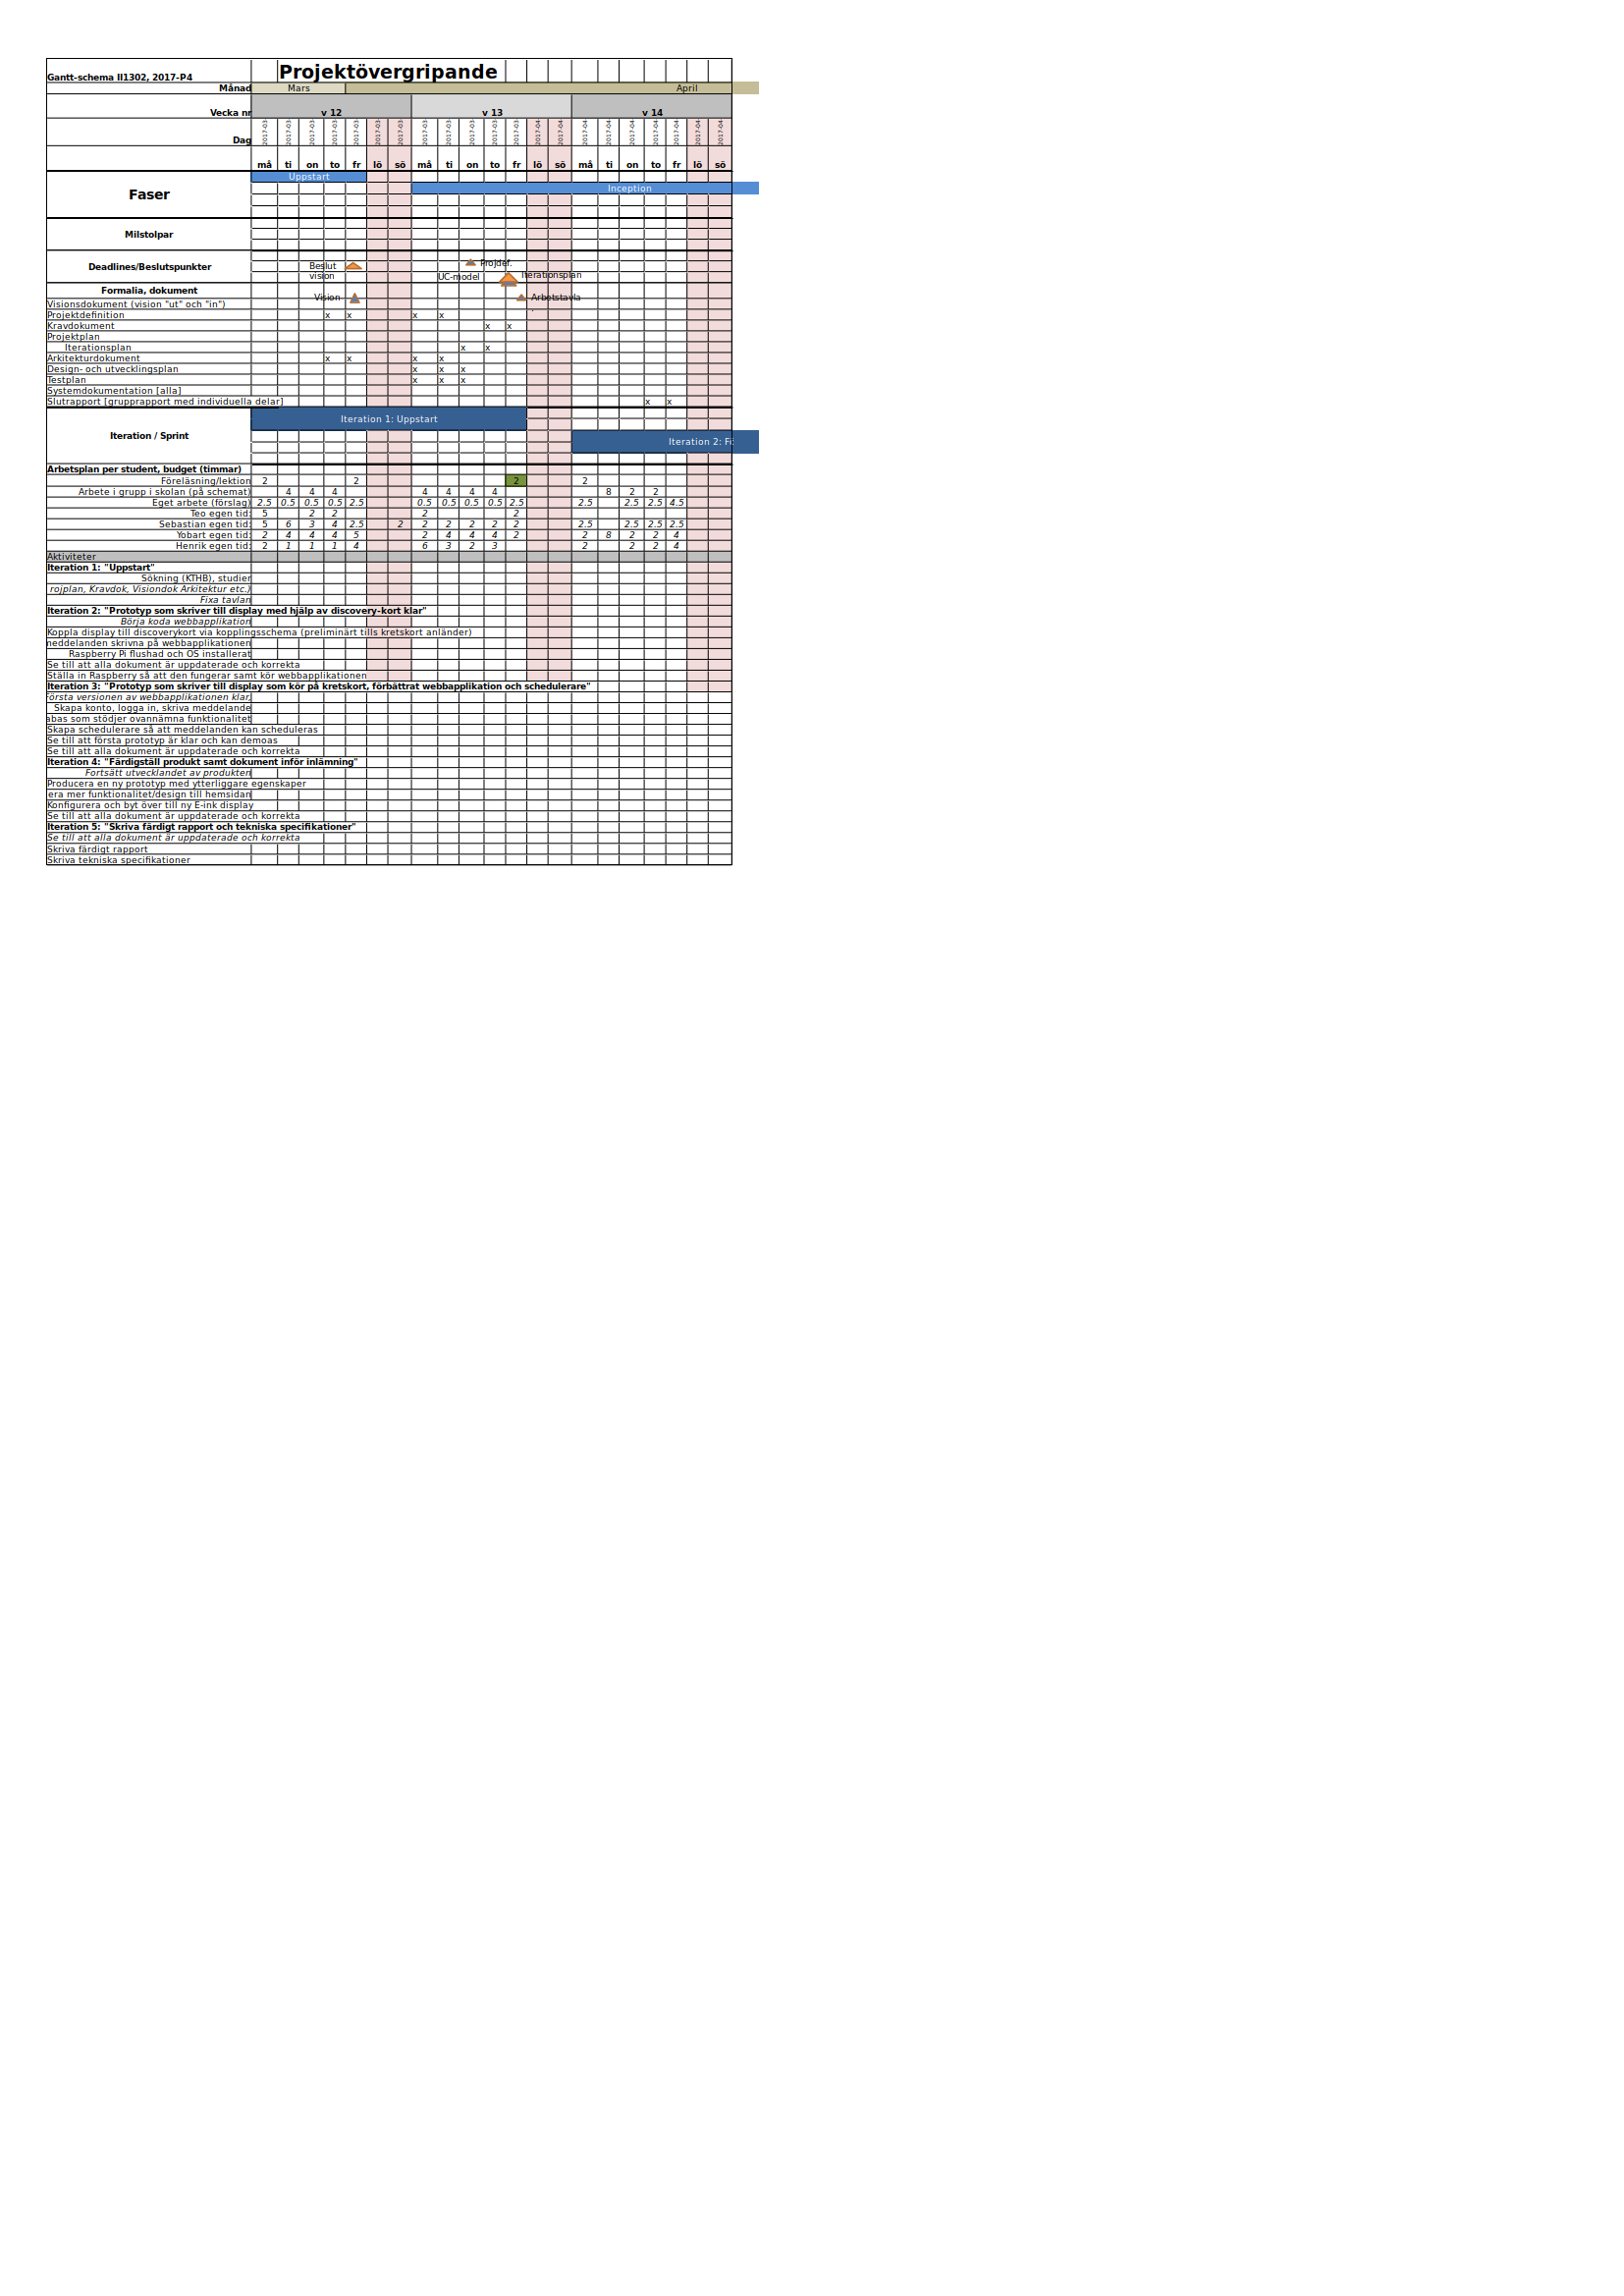
\includegraphics[width=.9\linewidth]{../GANTT.png}
\end{center}
\subsection{Projekttriangel}
\label{sec:org725a6f3}

Projekttriangeln består som bekant av 3 hörn, kostnad, tid och kvalitét. (Projektmallar.se)
I detta projekt har vi en hård deadline, eftersom projektet genomförs i samband med en kurs. Detta medför
att projektets varaktighet är hårt kontrollerad, vår arbetstid är också begränsad till runt
180-200 timmar, men arbetstiden är mer flexibel då gruppen vid motgångar kan jobba övertid
för att ro projektet i land.\\
$\backslash$\Projektets budget är ej så flexibel, då kursen består av många
projektgrupper som alla ska dela på kursens tillgångar. Den stora flexibiliteten i projekttriangeln
ligger i kvaliten, då grundkraven för produkten är små så är det här gruppen kommmer att behöva
bortprioritera i de fall vi hamnar efter och känner att vi håller på att gå utanför projekttriangeln.


\section{Intressenter}
\label{sec:org9f72431}
\begin{center}
\begin{tabular}{1 p{3cm} p{5cm} p{5cm}}
Inressent & Namn & Förväntningar & Uppfyllande av förväntningar\\
\hline
Examinator & Anders Sjögren & Att gruppmedlemmarna ska lära sig agila projektmetoder samt nå kursmålen så att de klarar kursen & Att lämna in en tillfredsställande slutprodukt, samt samtliga dokument under rubriken dokumentplan i denna projektdefinition där kursrapporten är det viktigaste dokumentet.\\
Uppdragsgivare & Anders Sjögren & Få en fungerande slutprodukt innan deadline & På ett planerat och strukturerat sätt utveckla samt leverera slutprodukten innan deadline.\\
Projektgrupp &  & Genom att genomföra ett planerat och strukturerat arbete lära sig mer och projektmetodik och få mer erfarenhet inom projektarbete för att förbereda inför kommande arbetsliv samt examensjobb. & Noga planera upp arbetet och strukturera detta planerande genom att skriva utförliga dokument som täcker all nödvändig information som krävs för att genomföra projektet på ett tillfredsställande sätt och samtidigt få mer kunskap kring projekt samt projektmetoder.\\
Skola & Kungliga Tekniska Högskolan & Att utbilda kompetenta ingenjörer och/eller forskare som sedan kan ta mark på arbetsmarknaden. & Genom att genomföra kursen till den grad att studenten får ett tillfredsställande betyg i denna kurs, likt alla andra kurser, på så sätt att studenten är attraktiv på arbetsmarknaden och därmed kan få ett jobb.\\
\end{tabular}
\end{center}

\section{Riskanalys}
\label{sec:orgff0654f}
Nedan beskrivs identifierade risker som finns i sprint 1 och 2, se
appendix B för riskanalys av sprint 3 och 4.

\begin{center}
\begin{tabular}{1 p{4cm} p{6cm} p{5cm}}
ID & Risk & Förebyggande åtgärd & Åtgärder vid riskutfall\\
\hline
R1 & Sjukdom & Genom att se till att alla projektmedlemmar bidrar till projektet undviker vi att någon projektmedlem överarbetar och därmed så minskar risken att någon medlem insjuknar. Eftersom alla är med och bidrar så har även alla medlemmar någorlunda koll på projektet och kan därför täcka upp för varandra. & Sjuka gruppmedlemmar skall arbeta till sin bästa förmåga hemifrån för att påskynda tillfrisknad samt undvika att sprida sjukdom till resterande gruppmedlemmar.\\
R2 & Tidsbrist & Planera upp projektet i sin helhet redan från start, använd denna plan i konjunktion med en agil arbetsprocess samt något hjälpmedel (i vårt fall en scrumboard) för att enkelt kunna se om planeringen efterföljs. & I fallet där gruppen hamnar efter planering så får gruppen tillsammans med uppdragsgivare komma överens om vilka delar av projektet som ska kompromissas så att projektet hinner klart i tid.\\
R3 & Leverans avHårdvara & Beställa hårdvaran från leverantörer som historiskt är kända för att uppfylla leveranskrav. & Ha backup kretskort som vi då själva får producera med hjälp av till exempel en fräs eller laser.\\
R4 & Förlust av kod & Använda GitHub för versionshantering. & GitHub innehåller en funktion där man kan gå tillbaka i versioner, och därmed få tillbaka äldre kod/data.\\
R5 & Samtliga medlemmar kan inte hantera samtliga delar av projektet & Olika medlemmar specificerar sig samt har tidigare erfarenheter av olika delar av projektet, och denna kunskap måste förmedlas till samtliga medlemmar genom dokumentation samt utbildning, på detta sätt minimerar vi risken att någon medlem försvinner och projektet därför blir stående. & Vid riskutfall ska tydlig dokumentation finnas tillgänglig så att medlemmar kan konsultera denna dokumentation och utifrån den genomföra delar projektet som personen I fråga kanske inte har specialiserat sig på\\
R6 & Medlemmar kommer ej överens och det bildas sprickningar I projektgruppen & Då första sprinten går ut mycket på att läsa teori och lära känna varandra så kastas gruppen ej in i hårt arbete direkt, därför har vi tid att lära känna varandra och känna av varandras styrkor och svagheter, och jobba för att alla ska känna att de har en plats i projektgruppen & Om gruppen verkligen ej kommer överens så finns inget annat alternativ än att försöka bryta upp gruppen och bilda nya grupper, detta går antagligen att ordna med kursansvarig och borde således ej vara ett problem, men det är verkligen ett värsta-fall scenario.\\
\end{tabular}
\end{center}

\subsection{Riskbedömning}
\label{sec:org9915f18}

\begin{center}
\begin{tabular}{|l|l|l|l|l|}
\hline
 & \multicolumn{3}{l|}{Hög sannolikhet} & \\
\hline
 & R4 & R2 & & \\
\cline{2-4}
Liten Påverkan & R1 & & R3, R5 & Stor påverkan \\
\cline{2-4}
 & & & & \\
\hline
 & \multicolumn{3}{l|}{Låg sannolikhet} & \\
\hline
\end{tabular}
\end{center}

\section{Kostnadsplan}
\label{sec:orgfe7cd6b}
Vilka kostnader finns i projektet? Vem betalar vad? Licenser?

\begin{center}
\begin{tabular}{1 1 1 p{5cm}}
Vad? & Betalas av? & Kostnad & Beskrivning\\
\hline
Frimärks-display & Anders Sjögren & Vet ej & Displayen som ska användas för meddelandet.\\
Wifi-modul (ESP8266) & Anders Sjögren & Cirka 100 :- & Wifi-modul som kopplas till displayen så att den kan kommunicera trådlöst med Raspberry.\\
Kretskort & Bengt Molin & Cirka 100 :- & Det kretskort som ska användas för att koppla displayen till Raspberry Pi.\\
E-ink display & Anders Sjögren & Cirka 500:- inkl frakt & En större display som använder bläck för att visa innehåll, denna display drar mindre ström och är lite roligare att hålla på med, planen är att gå över från frimärksdisplayen till denna och använda frimärksdisplayen för debug meddelanden etc.\\
Raspberry Pi v.3 & Lånas av Anders Sjögren & Fanns redan inköpt & Den Raspberry Pi som skall driva projektet, webbapplikationen skall köras på denna rasp och den ska vara kopplad via WiFi till displayen.\\
\end{tabular}
\end{center}

\section{Dokumentplan}
\label{sec:org12a75d8}
Vilka dokument skall användas, underhållas, granskas och levereras? När
skall detta ske och för vilka?

\begin{center}
\begin{tabular}{p{3cm} p{3cm} p{3cm} p{7cm}}
Namn & Ska underhållas? & Hur ofta? & Beskrivning\\
\hline
Projektdefinition & Ja & Varje sprint & Dokument som definierar projektet.\\
Iterationsplan & Ja & Varje vecka & Grovplanering över hela projektet.\\
Scrumboard & Ja & Varje Vecka & Tavla som ger en översikt över Scrumen.\\
Vision & Nej & - & Vår vision över projektet, skrivs i början av projektet och beskriver hur och varför vi ska genomföra projektet.\\
Kursrapport & Ja & Varje vecka from. Iteration 2-3 & Kursrapporten som ska lämnas in i slutet av kursen.\\
Tekniska specifikationer för olika komponenter i systemet (fyra stycken) & Nej, men ska dock skrivas i period 4 och 5 & - & Tekniska specifikationer som beskriver komponenter i systemet mer i detalj så att läsare antingen kan lära sig hur systemet fungerar eller få mer information så att de kan vidareutveckla systemet. (Upp till författaren att välja på vilken nivå specifikationen ska läggas)\\
\end{tabular}
\end{center}

\section{Utbildningsplan}
\label{sec:org865a1b8}
Behov av förstudie, inläsning, utbildning.

\begin{center}
\begin{tabular}{1 1 p{5cm} p{5cm}}
Namn & När? & Varför? & Beskrivning\\
\hline
Git intro & Sprint \#1 & För att vi ska använda Git i kursen. & En video-introduktion i Git som förklarar gruderna inom git, samt visar hur man sätter upp ett reposity och en wiki på webbsidan GitHub.\\
Handbok om Scrum, "Scrum and XP from the trenches" av Henrik Kniberg (Kniberg, 2007) & Sprint \#1 & För att vi ska jobba med Scrum i kursen. & En handbok som förklarar hur författaren jobbar med Scrum i skarpa IT-Projekt. Denna text skall ge oss en inblick i hur Scrum används och hur vi kan använda oss utav Scrum.\\
Handbok om KanBan, "Scrum and KanBan, get the best of both worlds" av Henrik Kniberg (Kniberg, 2010) & Sprint \#3 & Vi ska utöver Scrum även ha hört talas/ha lite kunskap om KanBan, som är en annan projektmetodik & Läsa Handbok om KanBan och Scrum som finns på kurswebben. Detta för att få ytterliggare\\
Artikel om Essence (Jacobson, 2016) & Sprint \#3 & Vi använder oss av Essence, som är ett hjälpmedel i form av kort samt tabeller som används i mjukvaru-utveckling & Läsa in sig på Essence då detta är något vi bestämt oss för att delvis tillämpa i projektet.\\
"Software Engineering" av Ian Sommerville (Sommerville, 2010) & Sprint \#1 & För att de tre första kapitlerna behandlar projektarbeten, främst inom mjukvaru-utveckling men samma principer gäller inom IT-projekt & De tre första kapitlerna ska läsas för att få mer information om IT-projekt\\
\end{tabular}
\end{center}

\section{Appendix A - Referenser}
\label{sec:orgb7174b9}
Andersson, N., \& Ekholm, A. (2002). Vetenskaplighet - Utvärdering av tre
implementeringsprojekt inom IT Bygg \&amp; Fastighet 2002.

Eklund, S. (2014). \emph{Arbeta i projekt: individen, gruppen, ledaren}:
Studentlitteratur.

Jacobson, I \& Spence, I \& Seidewitz, E. (2016). Industrial-scale Agile: From Craft to Engineering. \emph{Commun} no. 12. ACM

Kniberg, H. (2007). \emph{Scrum and XP from the Trenches}: C4Media.

Kniberg, H. (2010). \emph{Kanban and Scrum - Making the Most of Both}: C4Media.

Permana, Putu Adi Guna. 2015. “Scrum Method Implementation in a Software
Development Project Management.” \emph{International Journal of Advanced
Computer Science and Applications (Ijacsa)} 6 (9).
\url{doi:10.14569/IJACSA.2015.060927}.

Projekttriangel - Projektmallar.se URL:\url{http://www.projektmallar.se/projekttriangeln}

Sommerville, I. (2010). \emph{Software Engineering}: Addison-Wesley Publishing Company.
\end{document}
